\documentclass[]{interact}

\usepackage{setspace}
\usepackage[T1]{fontenc}
\usepackage{lmodern}
\usepackage[utf8]{inputenc}
\usepackage[british]{babel}
\usepackage{amsmath,amssymb,bm,booktabs,tabularx,array,microtype}
\usepackage[authoryear,round]{natbib}
\bibpunct[, ]{(}{)}{;}{a}{}{,}
\usepackage[hidelinks]{hyperref}
\usepackage{xspace}

\usepackage[acronym,nonumberlist,shortcuts]{glossaries}
\newcommand{\glscite}[1]{\glsentrylong{#1} \ifglshasfield{useri}{#1}{\citep[\glsentryshort{#1};][]{\glscurrentfieldvalue}}{}\glsunset{#1}}
\newcommand{\Glscite}[1]{\Glsentrylong{#1} \ifglshasfield{useri}{#1}{\citep[\glsentryshort{#1};][]{\glscurrentfieldvalue}}{}\glsunset{#1}}
\makenoidxglossaries
\newcommand{\glstitle}[1]{\glsentrytitlecase{#1}{long}~(\glsentryshort{#1})\glsunset{#1}}
\newacronym{dlanp}{DLAN-P}{planar DLAN configuration}
\newacronym{dlan}{DLAN}{dimension-specific local attention network}
\newacronym[user1={BrunsdonFotheringham-1996}]{gwr}{GWR}{geographically weighted regression}
\newacronym[user1={FotheringhamYang-2017,LuBrunsdon-2017}]{mgwr}{MGWR}{multiscale geographically weighted regression}
\newacronym[user1={HuangWu-2010}]{gtwr}{GTWR}{geographically and temporally weighted regression}
\newacronym[user1={LuHu-2025}]{gtdr}{GTDR}{geographical and temporal density regression}
\newacronym[user1={HuHarris-2024}]{hgwr}{HGWR}{hierarchical and geographically weighted regression}
\newacronym[user1={KordiFotheringham-2016}]{swim}{SWIM}{Spatially Weighted Interaction Models}
\newacronym[user1={DuWang-2020,WuDu-2020}]{gnnwr}{GNNWR}{geographically neural network weighted regression}
\newacronym[user1={WuWang-2021}]{gtnnwr}{GTNNWR}{geographically and temporally neural network weighted regression}
\newacronym[user1={DaiWu-2022,LiuLi-2024}]{gcnnwr}{GCNNWR}{geographically convolutional neural network weighted regression}
\newacronym{film}{FiLM}{feature-wise linear modulation}
\newacronym{gvi}{GVI}{green view index}
\newacronym{od}{OD}{origin--destination}
\newacronym{rmse}{RMSE}{root mean squared error}
\newacronym{mae}{MAE}{mean absolute error}
\newacronym{mse}{MSE}{mean squared error}
\newacronym{ols}{OLS}{ordinary least squares}
\newacronym{mlp}{MLP}{multilayer perceptron}
\newacronym{knn}{KNN}{nearest-neighbour search}
\newacronym{kde}{KDE}{kernel density estimation}
\newacronym{poi}{POI}{point of interest}
\newacronym{sd}{SD}{standard deviation}
\newacronym{ce}{CE}{carbon emissions in China}
\newacronym{wuhanod}{SIC}{subdistrict-level spatial interaction counts in Wuhan, China}
\newacronym{wuhanhp}{SHP}{second-hand housing prices in Wuhan, China}
\newacronym{gvid}{GVI}{green view index in Shanghai, China}

\newcommand{\R}{\mathbb{R}}
\newcommand{\train}{\mathcal{T}}
\newcommand{\cand}{\mathcal{C}}
\newcommand{\softmax}{\operatorname{softmax}}
\newcommand{\gelu}{\operatorname{GeLU}}
\newcommand{\lnorm}{\operatorname{LN}}
\newcommand{\pending}[1]{\par\smallskip\noindent\textbf{Draft completion item.} #1\par\smallskip}

\newcommand{\DLAN}{\gls{dlan}\xspace}
\newcommand{\GNNWR}{\gls{gnnwr}\xspace}
\newcommand{\GTNNWR}{\gls{gtnnwr}\xspace}
\newcommand{\GCNNWR}{\gls{gcnnwr}\xspace}
\newcommand{\GAgg}{GeoAggregator\xspace}
\newcommand{\COO}{\gls{ce}\xspace}
\newcommand{\WuhanOD}{\gls{wuhanod}\xspace}
\newcommand{\WuhanHP}{\gls{wuhanhp}\xspace}
\newcommand{\GVI}{\gls{gvid}\xspace}

\graphicspath{{figures/}}

\begin{document}
\setstretch{2.0}

\articletype{RESEARCH ARTICLE}
\title{Dimension-specific local attention for nonlinear regression in geographical and temporal spaces}
\author{
\name{Yigong Hu\textsuperscript{a}, Bohan Liu\textsuperscript{b}, Zidong Fang\textsuperscript{a}, Linfang Ding\textsuperscript{a}, and Binbin Lu\textsuperscript{c*}\thanks{CONTACT Binbin Lu. Email: binbinlu@whu.edu.cn}}
\affil{\textsuperscript{a}College of Geography and Remote Sensing, Hohai University, Nanjing, China;\\%
\textsuperscript{b}School of Geospatial Artificial Intelligence, East China Normal University, Shanghai, China;\\%
\textsuperscript{c}School of Remote Sensing and Information Engineering, Wuhan University, Wuhan, China}
}
\maketitle

\begin{abstract}
Spatial heterogeneity requires models that combine local information
with flexible relationships between attributes and responses.
This study proposes a dimension-specific local attention network (DLAN),
linking coordinate-specific bandwidths to reference retrieval and a Gaussian product prior.
A FiLM-modulated predictor combines local context with query covariates.
Four case studies use ten training seeds per reported configuration.
Regressors have 6,957 trainable parameters in \COO, WuhanHP and GVI,
and 7,069 in the reported WuhanOD comparison.
The WuhanOD DLAN restores attention width 12
and uses 512 reference candidates,
achieving mean test root mean squared error 565.28.
Relative to \GAgg, the reported DLAN configurations reduce mean error
by 57.81\%, 26.85\%, 2.99\% and 7.58\%
on \COO, WuhanOD, WuhanHP and planar GVI, respectively.
The WuhanOD mean advantage coexists with a higher median
and fewer paired seed wins;
its candidate-count experiment spans two machines.
Retained configuration comparisons distinguish the historical width-10 result,
the restored-width K1024 diagnostic and the selected K512 result.
The results establish useful reference-conditioned nonlinear prediction,
with capacity allocation, candidate support and execution protocol
as consequential determinants of performance.
\end{abstract}

\begin{keywords}
Spatial heterogeneity;
local attention;
coordinate-specific bandwidth;
nonlinear spatial regression;
geographical flows
\end{keywords}

\glsresetall

\section{Introduction}\label{sec:intro}
Spatial dependence and spatial heterogeneity are two well-known properties of geographical data~\citep{Tobler-1970,Anselin-1988,Goodchild-2004},
indicating that neighbouring observations can share information that is absent from the covariates of an individual record whilst relationships between a response and its covariates may change across locations.
These properties motivate spatially explicit analysis rather than an assumption of identical relationships throughout a study region.
\Glscite{gwr}, which estimates spatial heterogeneous relationship for each sample by borrowing information from nearby locations, is a comprehensive reflection of the two properties of geographical data.
The model generates location-specific regression coefficients via a weighted least-squares estimator with weights determined by distance to geographical neighbours and a pre-defined kernel function.
In the past decade, the \gls{gwr} model has been widely applied in fields such as environmental science,
epidemiology, urban planning and transportation~\citep{LuGe-2020a}.

However, the original \gls{gwr} is incompatible with spatio-temporal and spatial flow data,
and it overlooks the scale differences in covariates.
Addressing the first issue, \glscite{gtwr}, \glscite{swim},
and \glscite{gtdr} extend the \gls{gwr} framework to coordinate spaces of any combination of geographical and temporal dimensions.
In particular, \Gls{gtdr} provides a uniform framework based on dimension-specific bandwidths and density regression theory~\citep{HyndmanBashtannyk-1996} for multidimensional spatio-temporal data without limited to a specific data type,
thus provides a general but powerful solution.
but they adopts uniform scale for all covariates.
\Glscite{mgwr} solved this problem by assigning different spatial scales to different covariate relationships.
Nevertheless, these models still assume a linear relationship between the response and covariates,
which may be restrictive in many applications.
Some nonlinearity extensions based on machine learning have been proposed,
such as geographically weighted random forest~\citep{LuoYan-2022} and Geographical-XGBoost~\citep{Grekousis-2025}.

With the prevalence of deep learning, neural network-based models have also been proposed to capture the nonlinear relationships in geographical data,
such as \glscite{gnnwr}, \glscite{gcnnwr} and \GAgg~\citep{DengLi-2025a}.
\Gls{gnnwr} and its extension \glscite{gtnnwr} uses a neural network to learn the spatial distribution of relationships between the response and covariates to replace pre-defined kernel functions.
It uncompresses the global regression coefficients to each sample to obtain spatially varying coefficients.
\Gls{gcnnwr} constructs a regular spatial grid and represents each prediction location by a distance map containing its distances to the grid points.
A convolutional neural network extracts spatial features from this map and generates location-specific multipliers for the global OLS intercept and regression coefficients.
The resulting local coefficients are combined with the explanatory variables to produce predictions.
These two methods retain the linear form of the model, but learn complicated non-linear mapping to approximate the spatial heterogeneous relationships.
\GAgg further extends the framework for tabular spatial data by a Transformer architecture.
It uses Cartesian product attention to combine covariate and response representations,
incorporating a distance-based Gaussian bias to aggregate reference information into a local context for the query,
which is concatenated with the query's own attributes and passed through a nonlinear feed-forward network to predict the response directly.
All these approaches form part of a broader movement towards spatially explicit artificial intelligence and location representation~\citep{JanowiczGao-2020,MaiJanowicz-2022,ReichsteinCamps-Valls-2019}.
However, they do not explicitly consider the spatio-temporal data and the scale difference between dimensions.

Attention provides a useful connection between these neural models and the weighting principles of \gls{gwr}.
An attention mechanism computes query-dependent weights over reference observations and aggregates their values~\citep{BahdanauCho-2016,VaswaniShazeer-2023},
while the weighting scheme in \gls{gwr} also computes weights based on the spatial proximity of observations and aggregates their values by weighted least squares to estimate the outcome.
A normalised Gaussian geographical kernel is a special case of an attention distribution when its log weight is used as the attention score.
Considering \gls{gtdr} models coefficients varying across locations,
i.e., a field mapping coordinates to regression parameters,
it is natural to consider whether a neural attention mechanism can be used to learn a nonlinear mapping from coordinates to regression parameters,
and whether the learned mapping can be used to predict the response at new locations.
By keeping the dimension-specific scale parameter, the model could be extended to multidimensional coordinate spaces,
no matter spatio-temporal data, spatial flow, spatial-temporal flow,
an so on.

This study proposes \glstitle{dlan}, which combines bandwidth-adaptive reference retrieval,
coordinate-specific attention and a nonlinear conditional predictor.
The network retains content-dependent attention, so observations with comparable geographical proximity can make different contributions.
A \gls{film} predictor then uses the aggregated condition to modulate the relationship between query covariates and the response~\citep{PerezStrub-2018}.
The empirical analysis distinguishes predictive accuracy,
computational cost and transfer of the modelling construction across data structures.
Section~\ref{sec:model} introduces the model;
Section~\ref{sec:data} describes the data and evaluation;
Sections~\ref{sec:results} and~\ref{sec:discussion} present the results and their interpretation;
Section~\ref{sec:conclusion} concludes.

\section{Methodology}\label{sec:model}
\subsection{Observations and the reference-based prediction task}
Let an observation be $(\bm{x}_i,\bm{u}_i,y_i)$, where $\bm{x}_i\in\R^p$ contains covariates,
$\bm{u}_i\in\R^D$ locates the observation in a geographical--temporal space,
and $y_i\in\R$ is its response.
A planar point has $D=2$;
a space--time observation can have $D=3$;
a flow between planar endpoints has $D=4$.
Coordinate dimensions describe the support of an observation, whereas covariates describe its attributes.
Increasing $D$ and increasing $p$ therefore have different meanings.

The model predicts a query response using the query covariates and coordinates, together with a fixed labelled training bank,
\begin{equation}
 \hat y_i=f_\theta\!\left(\bm{x}_i,\bm{z}_i;
       \{(\bm{x}_j,\bm{z}_j,y_j):j\in\train\}\right),
 \qquad z_{ia}=\frac{u_{ia}-\mu_a}{s_a}.\label{eq:task}
\end{equation}
For newly prepared data, coordinate centres and scales are fitted to training observations.
Feature and response standardisation also use training data.
All four main experiments use their recorded training-only coordinate transformations.
Query responses never enter the reference bank.
During training, the focal row is excluded from its own candidate set.
These rules define a labelled-reference prediction task and the information available at deployment.

\subsection{Bandwidth-adaptive reference retrieval}\label{sec:retrieval}
For attention block $\ell$, head $h$ and coordinate $a$, define a positive scale
\begin{equation}
 b_{\ell ah}=\operatorname{softplus}(\rho_{\ell ah})+10^{-6}.
\end{equation}
For each query--reference pair, the retrieval score uses a coordinate-scaled squared distance,
\begin{equation}
 d^2_{\ell h}(i,j)=\sum_{a=1}^D
       \left(\frac{z_{ja}-z_{ia}}{b_{\ell ah}}\right)^2.
 \label{eq:distance}
\end{equation}
The candidate set is the deduplicated union of the $K$ closest eligible training references through \gls{knn} under every block--head metric,
\begin{equation}
 \cand_i=\bigcup_{\ell,h}\operatorname{TopK}_{j\in\train\setminus\{i\}}
                       \{-d^2_{\ell h}(i,j)\}.\label{eq:candidates}
\end{equation}
For an external query the exclusion applies only if a matching training-row identifier is supplied.
Candidate identifiers remain aligned across all coordinate projections.
Padding for a batch with variable candidate counts is masked before softmax.

This procedure selects points close under the current joint bandwidth metric.
It is different from taking a union of separate one-dimensional nearest-neighbour lists.
A reference close on one axis can remain distant under Equation~\eqref{eq:distance}.
The implementation refreshes candidates at each query microbatch using the current detached bandwidths.
Gradients update bandwidths through the attention score;
discrete candidate membership has no derivative.
With one block and one head there are at most $K$ candidates.
With multiple blocks and heads the union can contain up to $\min(N_{\train},LH K)$ distinct references,
where $L$ and $H$ are the numbers of blocks and heads.

\subsection{Content and response encoding}
Shared \gls{mlp} feature and coordinate encoders produce an observation token,
\begin{equation}
 \bm{e}_i=\lnorm\{E_x(\bm{x}_i)+E_z(\bm{z}_i)\}.
\end{equation}
The coordinate encoder uses Fourier features followed by a learned projection.
Fourier representations provide a means of expressing spatial variation at several frequencies~\citep{TancikSrinivasan-2020};
other location encodings, including rotary representations,
offer related ways to retain positional information~\citep{SuAhmed-2024,MaiJanowicz-2022}.
Query and key content are encoded without the query response.
For a reference, the value token additionally contains an encoding of its observed response,
\begin{equation}
 \bm{v}^{\rm in}_j=\bm{e}_j+E_y(y_j),\qquad j\in\train.
\end{equation}
Consequently, aggregation can convey information about both local attributes and locally observed outcomes.
Response encoding is a predictive information path;
it does not introduce a spatial-lag coefficient or a random effect.

\subsection{Dimension-specific scoring and joint attention}
Write $\delta_{ija}=z_{ja}-z_{ia}$.
Within one block, each coordinate and attention head has its own query, key and value projections.
The score is
\begin{align}
 s_{ihj}={}&\frac{1}{D}\sum_{a=1}^D
 \frac{(Q_{ah}\bm{e}_i)^\mathsf{T}(K_{ah}\bm{e}_j)}{\sqrt{d_h}}
 +\sum_{a=1}^D g_{ah}(\delta_{ija},|\delta_{ija}|,\operatorname{sgn}\delta_{ija})
 \nonumber\\[-2pt]
 &-\frac{1}{2}\sum_{a=1}^D
       \left(\frac{\delta_{ija}}{b_{ah}}\right)^2,
       \qquad j\in\cand_i,\label{eq:score}\\
 \alpha_{ihj}={}&\frac{\exp(s_{ihj})}{\sum_{r\in\cand_i}\exp(s_{ihr})}.
 \label{eq:attention}
\end{align}
The content scores are averaged across coordinates.
The log geographical kernels are summed.
The exponential of the final term is therefore a product of coordinate-specific Gaussian kernels,
\begin{equation}
 \exp\!\left[-\frac12\sum_a(\delta_{ija}/b_{ah})^2\right]
   =\prod_a \exp\!\left[-\frac{\delta_{ija}^2}{2b_{ah}^2}\right].\label{eq:product}
\end{equation}
The functions $g_{ah}$ represent learnt directional geographical biases.
Signed offsets allow an asymmetric contribution even though the Gaussian prior is symmetric.
The resulting attention need not decrease monotonically with distance because its content and bias terms can alter the score.

There is one softmax over the shared candidate identifiers for each query and head.
Separate coordinate projections do not produce separate coordinate-wise probability distributions.
The same weights aggregate every coordinate-specific value projection,
\begin{equation}
 \bm{c}_{iah}=\sum_{j\in\cand_i}\alpha_{ihj}V_{ah}\bm{v}^{\rm in}_j,
 \qquad
 \bm{c}_i=W_o\operatorname{concat}_{a,h}(\bm{c}_{iah})+\bm{b}_o.
\end{equation}
Residual connections, layer normalisation and a feed-forward network update the query representation,
yielding a local condition $\bm{h}_i$ after the final block~\citep{BaKiros-2016}.
Figure~\ref{fig:architecture} summarises the information paths.

\begin{figure}[tp]
\centering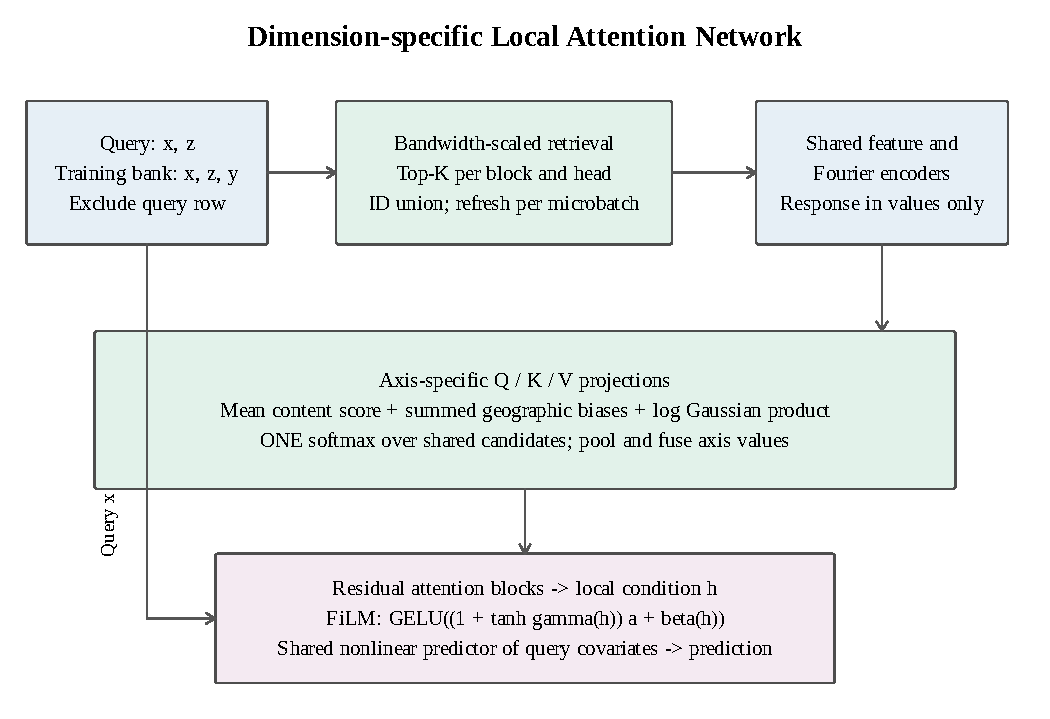
\includegraphics[width=\linewidth]{architecture.pdf}
\caption{The implemented DLAN architecture.
Bandwidths influence both candidate retrieval and Gaussian scoring.
Query responses are absent;
observed training responses enter value tokens.
The candidate union is across block--head metrics, followed by one shared candidate softmax per head.}\label{fig:architecture}
\end{figure}

The reference-pooling operation is also related to attention over graphs and unordered sets,
where learned weights combine contextual representations
\citep{VelickovicCucurull-2018,LeeLee-2019}.

\subsection{Conditionally modulated nonlinear prediction}
The response predictor retains a direct path from the query covariates.
Let $\bm{a}^{(r)}_i=W_r\bm{t}^{(r-1)}_i+\bm{c}_r$ with $\bm{t}^{(0)}_i=\bm{x}_i$.
The local condition modulates each hidden layer,
\begin{equation}
 \bm{t}^{(r)}_i=\gelu\!\left[
 \{1+\tanh(\bm{\gamma}_r(\bm{h}_i))\}\odot\bm{a}^{(r)}_i
       +\bm{\beta}_r(\bm{h}_i)\right].\label{eq:film}
\end{equation}
A final linear readout produces $\hat y_i$.
This use of \gls{film} allows the relationship between attributes and response to vary with the reference-derived condition~\citep{PerezStrub-2018}.
Houses at the same coordinates can receive different predictions because their individual covariates remain in the prediction path.
Nonlinear activations also permit attribute interactions and curved response functions.
The model does not estimate a collection of locally linear regression coefficients.

\subsection{Relationship to local regression and the planar configuration}
For \gls{gwr}, local calibration follows the weighted-regression construction
\citep{FotheringhamBrunsdon-2002},
with coefficient stability affected by local covariate collinearity
\citep{WheelerTiefelsdorf-2005,Wheeler-2007}.
The local estimate takes the form
\begin{equation}
 \hat{\bm{\beta}}(\bm{u}_i)
  =(X^\mathsf{T}W_iX)^{-1}X^\mathsf{T}W_i\bm{y}.
\end{equation}
If content and learnt geographical biases in Equation~\eqref{eq:score} are disabled,
Equation~\eqref{eq:attention} becomes a normalised geographical product kernel on its candidate support.
Pooling raw responses with those weights yields a local-constant kernel predictor,
connecting the attention construction to kernel and locally weighted regression
\citep{Nadaraya-1964,Watson-1964,Cleveland-1979}.
The product-kernel prior also inherits the coordinate-scale and smoothing choices
studied in kernel density estimation
\citep{Parzen-1962,Rosenblatt-1956,JonesMarron-1996}.
Recovering the \gls{gwr} estimator would additionally require the weighted least-squares solution above.
Thus shared geographical weighting does not make the estimators identical.
Similarly, DLAN borrows the coordinate-specific scale principle of \gls{gtdr},
but its nonlinear predictor is not a conditional density estimator.

For planar data, tying $b_x=b_y=b$ reduces the Gaussian product to
\begin{equation}
 \exp\!\left[-\frac{(\delta_x)^2+(\delta_y)^2}{2b^2}\right]
      =\exp[-\|\bm{z}_j-\bm{z}_i\|^2/(2b^2)].\label{eq:planar}
\end{equation}
This identity supplies an isotropic spatial prior.
A planar restriction, denoted \gls{dlanp}, can further tie spatial scales
and use joint spatial projections and Euclidean candidate retrieval,
whilst retaining the conditionally modulated nonlinear predictor.
These restrictions are additional choices;
setting $D=2$ alone leaves the dimension-specific projections and retrieval rule active.
The completed main comparison uses that unrestricted $D=2$ construction
for WuhanHP and GVI.
The planar restriction therefore explains the connection with conventional spatial locality,
rather than introducing a separate fitted model into the main results.

\subsection{Training and computation}
The neural models minimise mean squared error on training-standardised responses,
using AdamW and validation-based early stopping~\citep{LoshchilovHutter-2019}.
Validation chooses a checkpoint, and the test partition is used for the final assessment.
This follows the separation between fitting and predictive assessment underlying cross-validation and smoothing-parameter selection~\citep{Stone-1974,HurvichSimonoff-1998}.

With fixed candidate count $M$, attention on the candidates requires work proportional to $MDd$ per query for coordinate-specific value operations,
apart from projections and feed-forward processing.
However, the current candidate implementation evaluates distances to all $N_{\train}$ references for each block--head metric and uses a stable full sorting operation.
Its distance work is $O(LHN_{\train}D)$ and sorting is $O(LHN_{\train}\log N_{\train})$ per query.
The reduced attention support controls attention activation memory, but the retrieval stage still scans the training bank.
Query microbatching limits transient memory and gradient accumulation preserves the observation-weighted effective batch objective.
Computational scalability is therefore evaluated through both measured fit cost and these explicit algorithmic properties.

\section{Data and experimental design}\label{sec:data}

We use four cases to evaluate the proposed \DLAN and its competitors including \GNNWR, \GCNNWR, and \GAgg.
The empirical comparison comprises: 
(a) \COO;
(b) \WuhanOD;
(c) \WuhanHP;
and (d) \GVI.
They represent spatio-temporal data, spatial flow data, multilevel geographical data, and planar geographical data with remote sensing observations.
Importantly, \DLAN is able to cover all four cases, while all the competitors cannot under their originally implementations as they are mainly designed for planar geographical data.
To enable a fair comparison, \GNNWR actually represents \GNNWR and \GTNNWR for the spatio-temporal data and spatial flow data, respectively.
\GCNNWR has not been extended to spatial data, it only works on the geographical datasets, i.e., \WuhanHP and \GVI.
Both models did not work on the spatial flow data, i.e., \WuhanOD, due to the lack of a proper design for the flow data.
\GAgg is connected to an adaptor for the spatio-temporal and spatial flow data, which simply extends distance computation from planar coordinates to multidimensional coordinates to avoid essential changes to the original model.
Table~\ref{tab:data} summarises the data and fixed evaluation partitions.

\begin{table}[tb]
  \centering\small
  \caption{Data and fixed evaluation partitions.}
  \label{tab:data}
  \begin{tabular}{lrrrrrr}
    \toprule
    Case    & Samples & Covariates & Dimensions & Training & Validation & Test  \\
    \midrule
    \COO  & 13,000  & 8          & 3          & 9,732    & 1,643      & 1,625 \\
    WuhanOD & 13,807  & 35         & 4          & 9,618    & 2,104      & 2,085 \\
    WuhanHP & 19,599  & 17         & 2          & 15,475   & 2,196      & 1,928 \\
    GVI     & 2,122   & 176        & 2          & 1,696    & 213        & 213   \\
    \bottomrule
  \end{tabular}
\end{table}

\subsection{Data descriptions}

The \COO case use dataset collected from the repository of \citet{WuDu-2026} that provides a panel of 13,000 observations during 2014–2021 with 8 covariates covering population, economic growth, industrialization, and other aspects of county-level administrative units in China.
The whole data were divided into training, validation and test sets according to the year of observation:
observations from 2014--2019 form the training set,
2020 provides validation, and 2021 provides the test set.
Regions can occur in several years,
so the task is subsequent-year prediction for a panel of regions.
Coordinate, covariate and response transformations introduced by this experiment use training statistics.
The samples are located by $(x,y,t)$, where $x$ and $y$ are geographical coordinates and $t$ is the year.
This case compares models with a three-dimensional spatio-temporal regression problem.

The \WuhanOD case uses taxi-trajectory data collected in Wuhan from 20 to 26 July 2020.
The study area was restricted to subdistricts belonging to Wuchang, Hongshan and Qingshan districts.
Each passenger trip was assigned to its origin and destination subdistricts, and trips with the same ordered origin--destination (OD) pair were aggregated into an interaction count, forming a 4-D spatial dataset located by $(x_o,y_o,x_d,y_d)$,
In addition, seventeen \gls{poi} categories at each endpoint and average interaction length provide 35 covariates.
During the training, the model minimises error on a standardised $\log(1+y)$ target but
predictions are transformed back by $\max\{\exp(\hat y)-1,0\}$ before count-scale assessment.
The whole dataset are divided into training, validation and test sets with unordered endpoint pairs following the 70/15/15 grouped allocation.
The test therefore concerns held-out positive interactions within the observed geographical system.

The \WuhanHP case focus on a multilevel dataset, collected by \citet{HuHarris-2026}, that contains 19,599 second-hand housing observations at 776 communities in Wuhan, China.
Houses within one location share coordinates but have different attributes and responses.
It has 17 attributes describe floor category, decoration, building form, building area,
fees and access to schools, transport, retail, water and green land.
The dataset is divided into training, validation and test sets at the community level, with 15,475, 2196 and 1928 observations in each partition.
The test requires the geographical condition to transfer to unseen communities,
whilst the direct covariate path distinguishes individual dwellings.

The \GVI case focus on predicting \gls{gvi} that measures the visible share of greenery in street-level scenes and provides a human-scale description of the urban environment~\citep{LiZhang-2015,BiljeckiIto-2021}.
Its relationship with built-environment attributes can involve thresholds,
saturation and interactions that are poorly represented by a single linear response surface.
We collected street-view images in Shanghai, China and computed the \gls{gvi} via a model trained on manually labelled images.
Then, at the location where street-view images were taken, we downloaded the on-site remote sensing data from Sentinel-1 and Sentinel-2 satellites and cut them into patches.
We further collected the building-height, road-network density, categorical \gls{poi} counts, sky-view factors and canopy features from the same area.
It comprise 2,122 Shanghai-area observations captured during 2019--2022.
All the features are processed by a encoder to produce 176 covariates as model inputs.
This case is intended to examine the nonlinear prediction component related to features learnt from remote sensing data.

\subsection{Model settings}

\COO, \WuhanHP and \GVI retain the 6,957-parameter configurations.
\WuhanOD reports the restored-width \DLAN at 7,069 parameters and K512,
with \GAgg and \GNNWR at the same 7,069-parameter budget.
The complete earlier 6,957-parameter WuhanOD group remains archived
and is used only in the allocation diagnostic.
DLAN and \GAgg are evaluated on all four cases;
GCNNWR is evaluated on WuhanHP and GVI,
where its two-dimensional proximity grid applies.
The completed PyTorch baselines use GTNNWR for the three-coordinate \COO case
and GNNWR for WuhanOD, WuhanHP and GVI.
WuhanOD GNNWR retains all four endpoint coordinates in its distance input.

The GNNWR and GTNNWR networks are taken from the upstream PyTorch implementation,
pinned to commit \texttt{2711bdee9821bfe242992d2eb885a78be1cf2628}.
The adapters retain its spatially weighted neural network,
its spatio-temporal proximity network for GTNNWR,
and coefficient-wise modulation of fixed training-only OLS estimates.
GNNWR receives distances to fixed training-coordinate reference points;
GTNNWR receives separate spatial Euclidean distances and absolute year differences,
which its proximity network combines before coefficient modulation.
The four reported configurations use 128, 119, 134 and 134 references
for \COO, WuhanOD, WuhanHP and GVI, respectively.
References are chosen by deterministic coordinate-only farthest-point coverage
within the training partition.
Distances are standardised using training pairs or reference columns,
following the corresponding upstream input construction.
The reference counts and real network widths enforce the fixed parameter budget;
the experiment does not reproduce an unlimited full-reference configuration
or the upstream default optimisation schedule.

Architectural widths are selected by parameter arithmetic,
without validation or test scores determining the allocation
(Table~\ref{tab:widths}).
No unused parameters are added to reach the budget.
The frozen GVI encoder and fitted OLS buffers are outside the trainable count.
Equal trainable capacity therefore does not imply equal deployment storage,
internal parameter allocation or access to reference information.

\begin{table}[tb]\centering
\caption{Widths of the reported configurations.
WuhanOD uses 7,069 parameters; the other cases use 6,957.
DLAN and \GAgg entries give token width and two prediction-head widths.
GCNNWR entries give two convolution widths, pooled-grid side and hidden width.
The last column gives the two spatial-weight-network hidden widths;
\COO additionally uses a $2\to7\to1$ proximity network.}\label{tab:widths}
\small\setlength{\tabcolsep}{4pt}
\begin{tabular}{lrrrr}\toprule
Case & DLAN & \GAgg & GCNNWR & GNNWR / GTNNWR\\\midrule
\COO & $(13,12,24)$ & $(48,14,22)$ & -- & $(40,32)$\\
WuhanOD & $(12,10,8)$ & $(48,6,16)$ & -- & $(51,9)$\\
WuhanHP & $(14,20,17)$ & $(32,62,14)$ & $(5,16,2,73)$ & $(44,14)$\\
GVI & $(7,12,58)$ & $(32,7,11)$ & $(8,17,2,22)$ & $(31,12)$\\\bottomrule
\end{tabular}\end{table}

All configurations minimise training-standardised target \gls{mse} with AdamW,
learning rate 0.001 and weight decay 0.0001.
The effective batch size is 1,024,
with query microbatches of 64 and observation-weighted gradient accumulation.
Training runs for at most 300 epochs,
with validation \gls{mse} patience 30, minimum improvement $10^{-5}$,
a common learning-rate scheduler and gradient clipping.
Coordinate axes are standardised using training statistics;
feature and target scalers also use training rows only.
GNNWR and GTNNWR retain the upstream PReLU, batch normalisation and dropout construction.

DLAN retains bandwidth-adaptive retrieval, coordinate-specific projections,
one joint candidate softmax and the FiLM nonlinear predictor in all cases.
The reported DLAN candidate limits are 768 for \COO,
512 for WuhanOD and 512 for each planar case.
The restored-width K1024 and K2048 records remain separate sensitivity configurations.
\GAgg uses 256 joint-Euclidean neighbours,
Cartesian product attention and coordinate-preserving rotary encoding.
GCNNWR uses a $16\times16$ grid fitted to training-coordinate bounds,
training-reference distance statistics and training-only global OLS coefficients.

The inference information conditions differ by construction.
DLAN and \GAgg aggregate training-reference attributes, coordinates and responses,
excluding the focal row during training.
GNNWR and GTNNWR use reference coordinates and fitted training OLS coefficients;
GCNNWR uses its fitted proximity grid and OLS coefficients.
Their reference inputs do not carry individual training responses during prediction.
The comparison evaluates these complete systems under common data and optimisation controls.

\subsection{Supplementary configurations}
The WuhanOD capacity experiment has a separate 7,069-parameter budget.
DLAN uses attention width 12 and hidden prediction widths $(10,8)$,
in place of width 10 and $(36,3)$ in the archived 6,957-parameter group.
\GAgg is separately matched to 7,069 parameters,
with width 48 and prediction widths $(6,16)$.
The GNNWR comparison uses 119 training-coordinate references
and hidden widths $(51,9)$ at the same budget.
Each configuration has ten completed seeds.
This experiment changes capacity allocation as well as total capacity.
The reported WuhanOD configuration draws its comparators from this budget group,
and uses the subsequently completed K512 DLAN result.

A further ten-seed DLAN experiment increases attention width from 12 to 16,
retaining the $(10,8)$ head and $K=1,024$.
Its 10,773 parameters represent an unmatched increase in capacity.
The candidate-support experiment retains width 12 and 7,069 parameters,
with complete ten-seed runs at $K=512$ and $K=2,048$.
These two runs were executed on another computer with PyTorch 2.14.1;
the reused $K=1,024$ baseline used PyTorch 2.13.0 on the original machine.
The results describe exploratory support sensitivity,
with the cross-machine difference retained in their interpretation.
The incomplete four-seed $K=256$ record is excluded.

The GVI three-coordinate experiment adds elapsed capture month since January 2019
as a third coordinate.
All 2,122 observations, 176 fixed features, responses and spatial partitions
remain identical to the planar experiment.
DLAN and \GAgg each have ten completed seeds and 6,957 parameters.
To retain the budget, their widths change to $(6,16,33)$ and $(24,14,31)$;
DLAN's reference limit also increases from 512 to 768.
This is a parameter-matched configuration comparison on a fixed spatial split,
not a fixed-width temporal ablation or future-month holdout.

\subsection{Metrics and saved-output audit}
Prediction accuracy is measured by
\begin{align}
 \operatorname{RMSE}&=\sqrt{n^{-1}\sum_i(y_i-\hat y_i)^2},&
 \operatorname{MAE}&=n^{-1}\sum_i|y_i-\hat y_i|,\\
 R^2&=1-\frac{\sum_i(y_i-\hat y_i)^2}{\sum_i(y_i-\bar y)^2}.&&
\end{align}
Values are means of run-specific metrics;
$\pm$ denotes sample standard deviation across ten training seeds.
Medians, worst-seed errors and paired win counts accompany comparisons
where seed-sensitive outliers change the ordering.
The partitions are fixed within a case,
so seed variation describes optimisation sensitivity rather than independent geographical replication
\citep{RobertsBahn-2017,ValaviElith-2019,Brenning-2012}.
For WuhanHP, equal-community error is
\begin{equation}
 \operatorname{RMSE}_{\rm community}
 =\left\{G^{-1}\sum_{g=1}^{G}n_g^{-1}
           \sum_{i\in g}(y_i-\hat y_i)^2\right\}^{1/2}.
\end{equation}

The reported comparison comprises 140 completed fits and 280 saved validation/test prediction arrays.
It selects the stated configurations from the audited historical and supplementary records;
this selection does not represent an additional set of fits.
The completed supplementary configurations add 80 fits and 160 arrays.
For this revision, every array was checked against the fixed row identifiers,
responses, configuration digest and reported RMSE, MAE and $R^2$.
Checkpoint state and saved reload-audit records were also checked.
Twenty prediction arrays from ten historical HPC fits were audited separately,
retaining their distinct preprocessing and execution environment.
The analysis reads existing results without retraining.

For GVI, a nonspatial linear diagnostic is recovered from the OLS coefficients
already fitted and stored in GCNNWR checkpoints.
It is identical across seeds and is not counted as another neural configuration.
All quantitative figures are generated in R from the audited records.
Historical joint-attention Gaussian ablations remain separate
from the final-model configuration experiments.

\section{Experimental results}\label{sec:results}
\subsection{Accuracy across the four cases}
The reported comparison uses the restored WuhanOD DLAN configuration
and the corresponding 7,069-parameter baseline group
(Table~\ref{tab:accuracy}).
DLAN has the lowest mean RMSE on all four cases in these reported configurations.
Relative to \GAgg,
mean RMSE falls by 57.81\% for \COO,
26.85\% for WuhanOD, 2.99\% for WuhanHP and 7.58\% for GVI.
The WuhanOD result is K512 with attention width 12;
it is not the superseded 6,957-parameter configuration.
Figure~\ref{fig:relative} shows the seed-level distributions of test RMSE and MAE,
with each case occupying one row
and the two metrics displayed in separate columns.

\begin{table}[tb]\centering
\caption{Reported test results, ten seeds per configuration.
WuhanOD uses restored attention width 12 and K512 for DLAN,
with the separately matched 7,069-parameter comparator group.
K512 was trained on the second machine.
RMSE is mean $\pm$ sample SD; MAE and $R^2$ are seed means.}\label{tab:accuracy}
\small\setlength{\tabcolsep}{3.3pt}\begin{tabular}{llrrrr}\toprule
Case & Model & Parameters & RMSE & MAE & $R^2$\\\midrule
\COO & DLAN & 6,957 & $0.2910\pm0.1076$ & 0.2259 & 0.9338\\
 & \GAgg & 6,957 & $0.6897\pm0.0182$ & 0.5064 & 0.6688\\
 & GTNNWR & 6,957 & $0.8986\pm0.0894$ & 0.6797 & 0.4332\\
\midrule
WuhanOD & DLAN & 7,069 & $565.28\pm154.31$ & 50.28 & 0.9051\\
 & \GAgg & 7,069 & $772.73\pm835.04$ & 60.19 & 0.6592\\
 & GNNWR & 7,069 & $3568.80\pm969.21$ & 210.94 & -2.7794\\
\midrule
WuhanHP & DLAN & 6,957 & $0.1656\pm0.0041$ & 0.1254 & 0.6080\\
 & \GAgg & 6,957 & $0.1707\pm0.0030$ & 0.1310 & 0.5836\\
 & GNNWR & 6,957 & $0.1702\pm0.0020$ & 0.1300 & 0.5858\\
 & GCNNWR & 6,957 & $0.1718\pm0.0019$ & 0.1289 & 0.5784\\
\midrule
GVI & DLAN & 6,957 & $0.0985\pm0.0038$ & 0.0760 & 0.3306\\
 & \GAgg & 6,957 & $0.1066\pm0.0051$ & 0.0831 & 0.2157\\
 & GNNWR & 6,957 & $0.1258\pm0.0255$ & 0.0987 & -0.1320\\
 & GCNNWR & 6,957 & $0.1185\pm0.0001$ & 0.0944 & 0.0318\\\bottomrule\end{tabular}\end{table}

\begin{figure}[tp]\centering
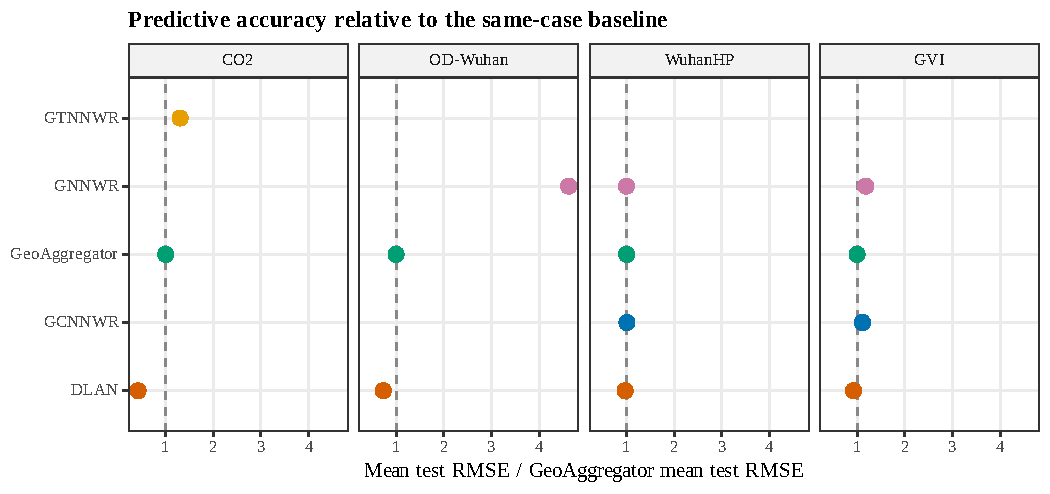
\includegraphics[width=\linewidth]{matched_relative_accuracy.pdf}
\caption{Distributions of test RMSE (left column) and MAE (right column) across ten training seeds.
Rows correspond to \COO, WuhanOD, WuhanHP and GVI.
Boxes show the interquartile range,
with the median marked by the central line
and whiskers extending to the most extreme observations within 1.5 interquartile ranges of the box.
Points show all ten seeds for each model.
The two metrics share a vertical scale within each row,
with separate vertical scales across datasets.
WuhanOD uses 7,069 parameters and the other cases use 6,957.
The DLAN WuhanOD results use attention width 12 and K512.}\label{fig:relative}
\end{figure}

The added baselines preserve DLAN's leading mean ranking in the three previously favourable cases.
Its RMSE is 67.62\% below GTNNWR on \COO,
2.74\% below GNNWR on WuhanHP and 21.75\% below GNNWR on GVI.
DLAN wins all ten paired seeds against GTNNWR on \COO,
nine against GNNWR on WuhanHP and all ten against GNNWR on GVI.
Against \GAgg it wins ten, eight and ten seeds in these cases,
and four of ten WuhanOD seeds.
The reported 7,069-parameter GNNWR has negative test $R^2$ in every WuhanOD seed
and in four GVI seeds under the controlled reference budget.
These are outcomes of the evaluated reference counts and common training protocol,
rather than estimates of each model family's fully tuned performance limit.

\begin{figure}[tp]\centering
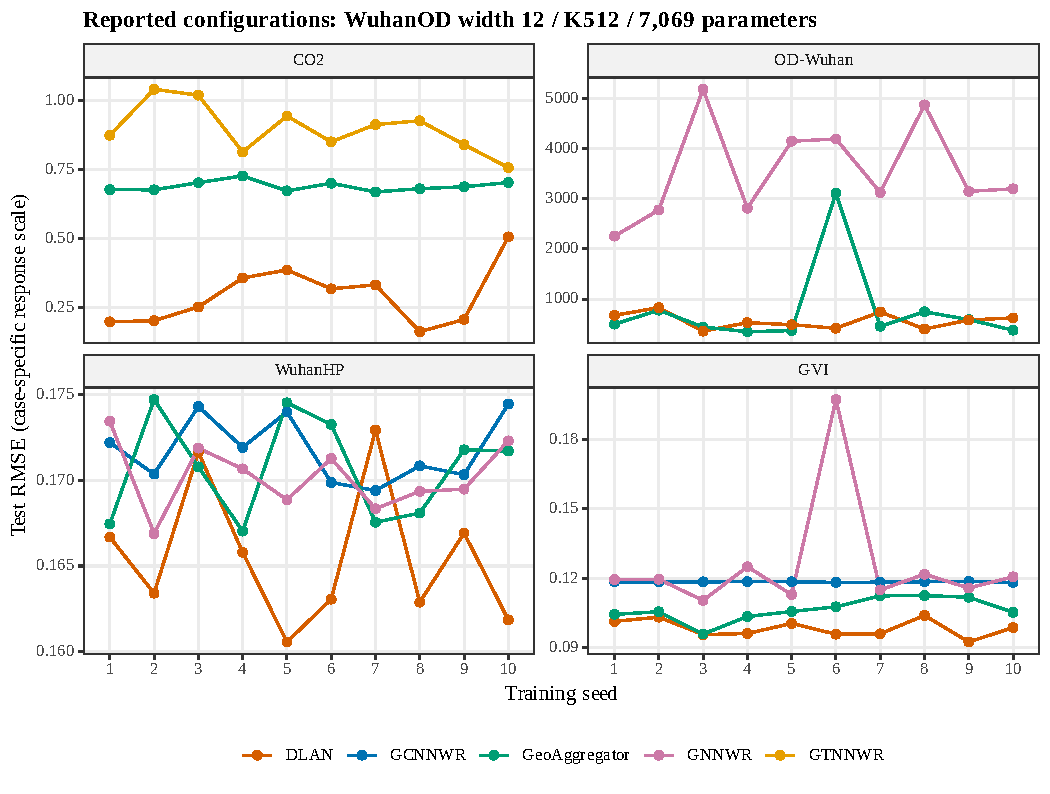
\includegraphics[width=\linewidth]{matched_seed_accuracy.pdf}
\caption{Test RMSE for the 140 reported fits.
Models share the same partition within each case;
WuhanOD K512 spans an execution environment different from its comparators;
y-axis response scales differ across cases.}\label{fig:seeds}
\end{figure}

\subsection{Future-year \texorpdfstring{\COO}{CO2} prediction}
DLAN's mean RMSE is 0.2910,
compared with 0.6897 for \GAgg and 0.8986 for GTNNWR.
Mean $R^2$ is 0.9338, 0.6688 and 0.4332, respectively.
DLAN improves on both alternatives in every paired seed.
Its RMSE range is 0.1610--0.5055,
compared with 0.6690--0.7271 for \GAgg.
Thus the larger DLAN seed variation does not reverse the ordering
in any run of this experiment.
Figure~\ref{fig:co2pred} shows seed-1 predictions and residuals,
using the same identifier-fixed example for every model.

\begin{figure}[tp]\centering
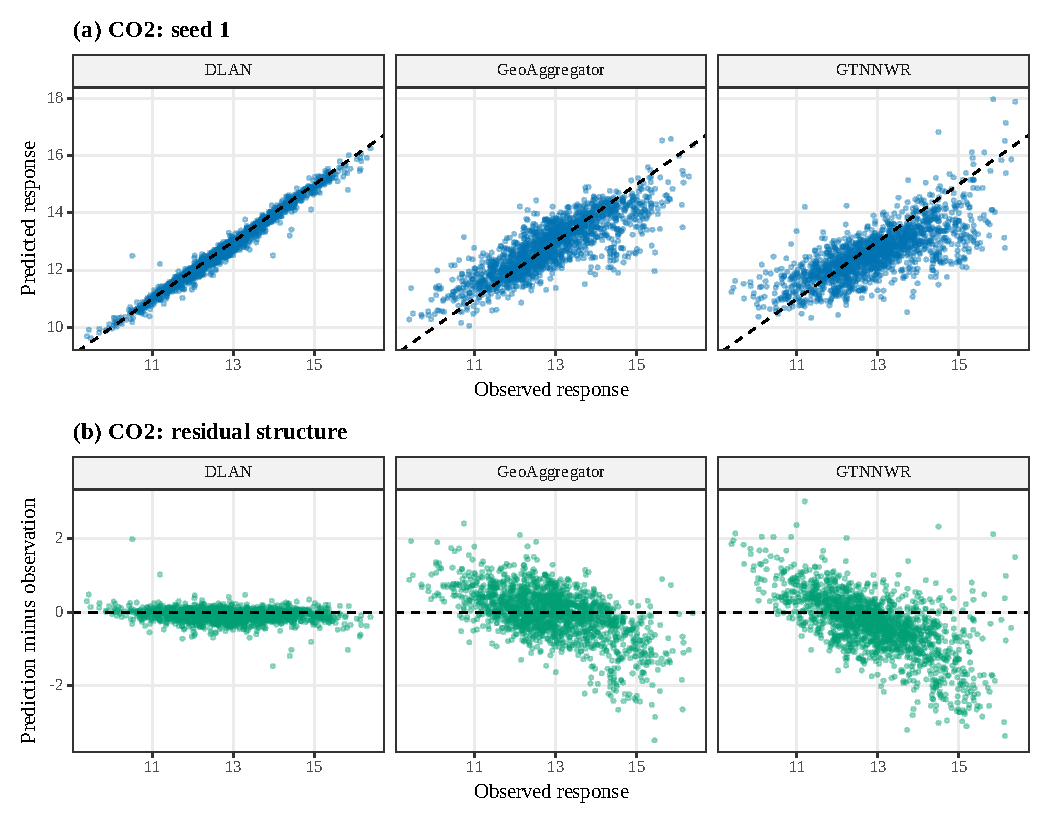
\includegraphics[width=\linewidth]{matched_co2_predictions.pdf}
\caption{\COO test predictions and residuals for seed 1,
on the same 1,625 held-out observations from 2021.
Dashed lines indicate perfect prediction and zero residual.}\label{fig:co2pred}
\end{figure}

The mean DLAN bandwidths are 0.0683 for spatial $x$,
0.0793 for spatial $y$ and 0.1860 for time
(Figure~\ref{fig:bandwidths}).
The Gaussian prior therefore decays more slowly in the transformed temporal coordinate
than in either spatial direction.
GTNNWR also learns a nonlinear combination of spatial and temporal proximity,
but its response remains an OLS coefficient-modulation construction.
DLAN additionally retains a nonlinear covariate predictor conditioned on labelled training references.
The results establish a predictive difference between these complete constructions;
they do not isolate one information path as the cause of the improvement.

\begin{figure}[tp]\centering
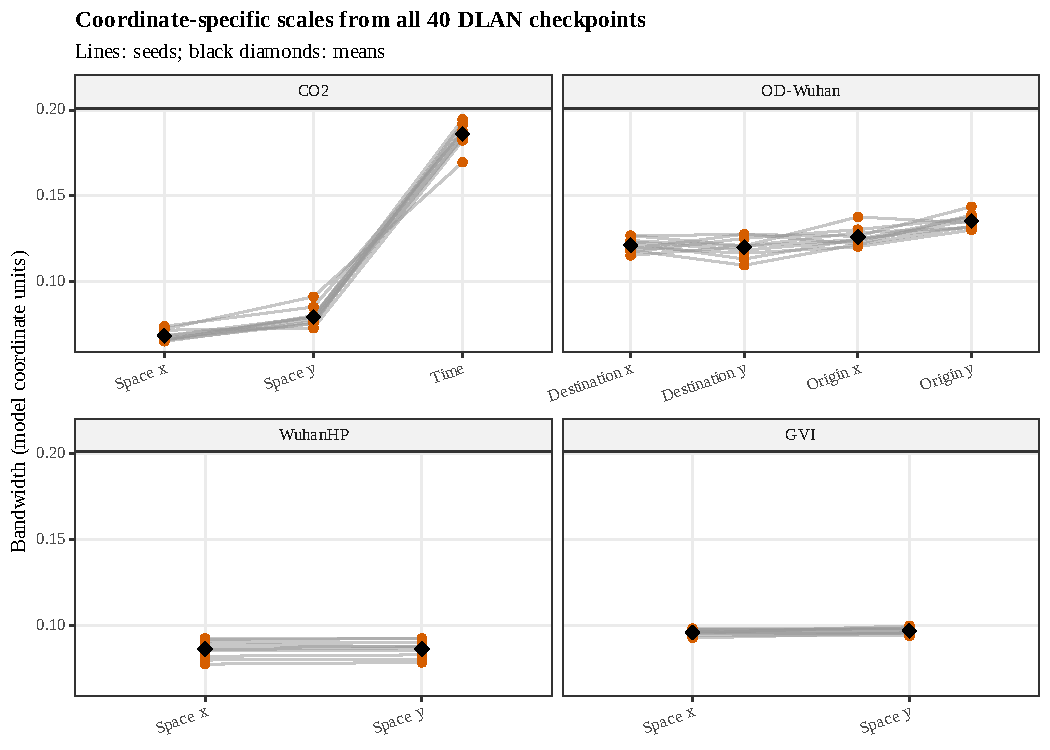
\includegraphics[width=\linewidth]{matched_bandwidths.pdf}
\caption{Coordinate-specific scales from all 40 reported DLAN checkpoints.
WuhanOD uses the width-12 K512 checkpoints.
Lines connect scales within a seed;
black diamonds indicate means in model-coordinate units.}\label{fig:bandwidths}
\end{figure}

\subsection{WuhanOD: restored attention width and selected candidate support}\label{sec:odcapacity}
The reported WuhanOD DLAN uses attention width 12,
prediction-head widths $(10,8)$ and 512 actual training-reference candidates.
Its 7,069 trainable parameters are unchanged by candidate count.
Across ten seeds, mean test RMSE is 565.2762909669982 counts,
with sample SD 154.3069,
mean MAE 50.2819 and mean $R^2=0.9051$.
The corresponding $K=2,048$ result is $587.60\pm171.15$,
not 565.28.
The reported DLAN configuration is therefore the completed $K=512$ experiment.

Against the separately matched 7,069-parameter comparators,
DLAN's mean RMSE is 26.85\% below \GAgg's 772.73
and 84.16\% below GNNWR's 3,568.80.
This corrects the earlier presentation of the superseded width-10,
6,957-parameter result of 919.92 as the main DLAN score.
That earlier allocation remains a configuration diagnostic,
not the reported final model.

The lower mean does not imply better prediction in most seed pairs.
For the reported $K=512$ model, median RMSE is 556.20,
compared with 478.91 for \GAgg;
DLAN wins four of ten pairs.
\GAgg has one severe run with RMSE 3,110.57,
whereas the selected DLAN's worst run is 827.76.
The reported mean advantage therefore coexists with a higher median
and a smaller observed extreme error.
No seed is omitted.
These configurations also span execution environments:
the K512 model was trained on the second computer,
whilst the comparator runs were recorded on the original machine.

The retained capacity experiment explains the sequence of model configurations
(Table~\ref{tab:odcapacity}).
At $K=1,024$, restoring attention width from 10 to 12
and changing the prediction head from $(36,3)$ to $(10,8)$
reduces mean RMSE from 919.92 to 608.73.
The subsequent completed support experiment yields 565.28 at $K=512$.
These are three distinct records;
608.73 is the restored-width K1024 diagnostic,
and 919.92 is the historical narrower-allocation score.

\begin{table}[tb]\centering
\caption{Restored-width WuhanOD comparison at K1024 and 7,069 parameters,
retained as a capacity diagnostic.
The reported DLAN model instead uses K512, as shown in Table~\ref{tab:accuracy}.}\label{tab:odcapacity}
\small\begin{tabular}{lrrrr}\toprule
Model & RMSE & Median RMSE & MAE & $R^2$\\\midrule
DLAN, K1024 & $608.73\pm252.45$ & 552.52 & 52.08 & 0.8809\\
\GAgg & $772.73\pm835.04$ & 478.91 & 60.19 & 0.6592\\
GNNWR & $3568.80\pm969.21$ & 3171.19 & 210.94 & -2.7794\\
\bottomrule\end{tabular}\end{table}

The capacity reallocation increases attention-block parameters
from 3,268 to 4,368,
whilst reducing nonlinear-head parameters from 2,269 to 925.
It improves mean RMSE in eight of ten paired seeds,
but changes both head structure and attention width.
Figure~\ref{fig:odcapacity} retains the two complete historical allocation groups;
it is not the primary selected-support ranking.

\begin{figure}[tp]\centering
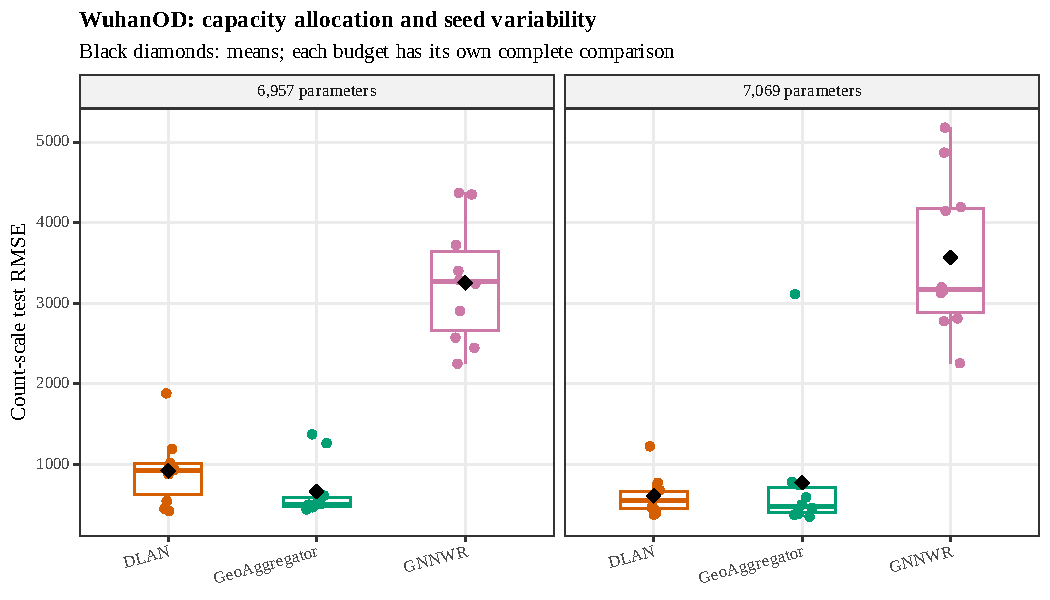
\includegraphics[width=\linewidth]{od_capacity_stability.pdf}
\caption{Historical WuhanOD allocation comparison at K1024,
with separately matched budgets of 6,957 and 7,069 parameters.
The selected K512 DLAN is evaluated separately in the primary results.}\label{fig:odcapacity}
\end{figure}

For the reported model, the largest 1\% of observed test flows
contribute on average 97.43\% of DLAN's squared error,
compared with 98.28\% for \GAgg.
After excluding this tail,
DLAN's remaining-count RMSE is 85.39 versus 65.88 for \GAgg.
Thus its smaller overall mean RMSE does not represent uniformly lower error
throughout the response distribution.
Figure~\ref{fig:odtail} uses the selected K512 predictions
and the corresponding 7,069-parameter baseline records.

\begin{figure}[tp]\centering
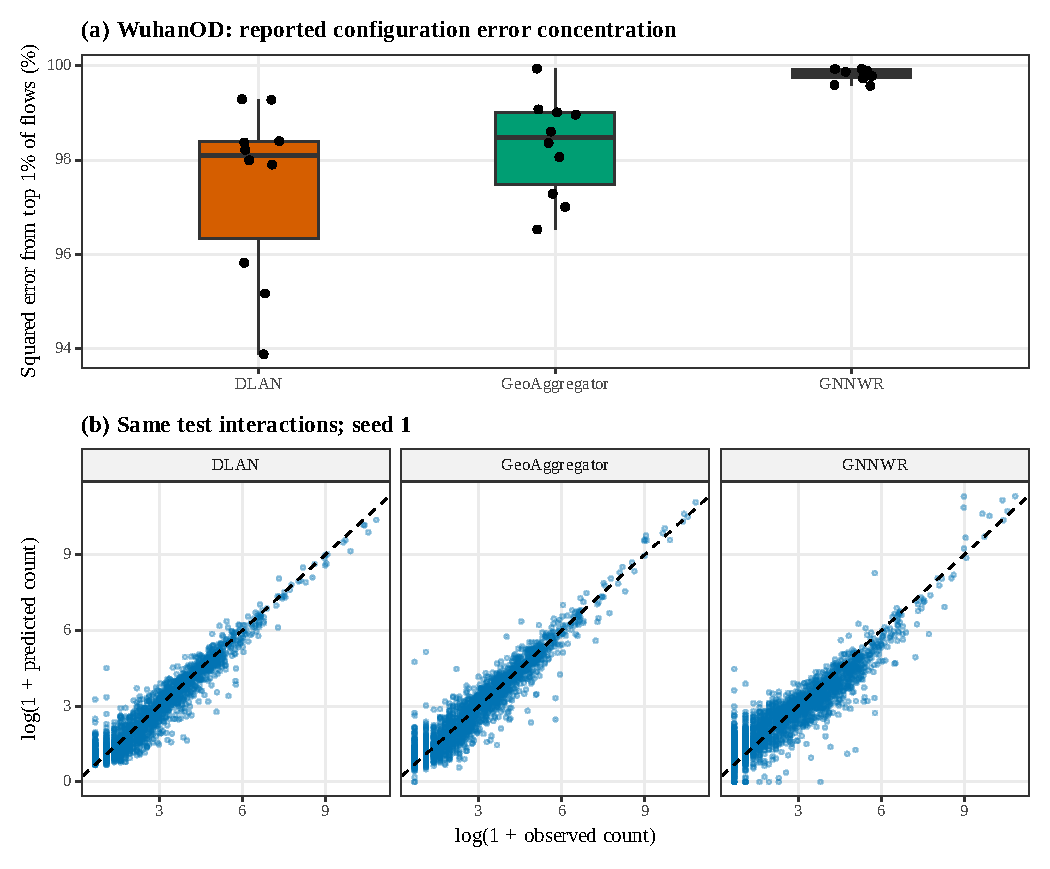
\includegraphics[width=\linewidth]{matched_od_tail.pdf}
\caption{Response-tail diagnostics for the reported WuhanOD configurations:
DLAN width 12 with K512 and the 7,069-parameter comparators.
Top: squared-error share from the largest 1\% of observed counts.
Bottom: seed-1 predictions on logarithmic axes.}\label{fig:odtail}
\end{figure}

\subsection{WuhanHP: prediction at unseen communities}
DLAN has mean RMSE 0.1656,
compared with 0.1702 for GNNWR, 0.1707 for \GAgg
and 0.1718 for GCNNWR.
Its error reductions are 2.74\%, 2.99\% and 3.60\%, respectively.
It wins nine paired seeds against GNNWR,
eight against \GAgg and nine against GCNNWR.
Mean MAE and $R^2$ give the same ordering.
The added GNNWR baseline performs similarly to \GAgg,
but does not change DLAN's leading mean accuracy.

DLAN's equal-community RMSE is 0.1629,
compared with 0.1695 for GNNWR,
0.1699 for \GAgg and 0.1722 for GCNNWR.
The ranking persists when each held-out community receives equal weight.
Figure~\ref{fig:hpgroups} shows community residuals and errors by group size,
averaged over ten seeds.
The model combines a reference-derived geographical condition
with individual housing attributes,
so dwellings sharing coordinates can still receive different predictions.
Test communities have no labelled observations in the training-reference bank.

\begin{figure}[tp]\centering
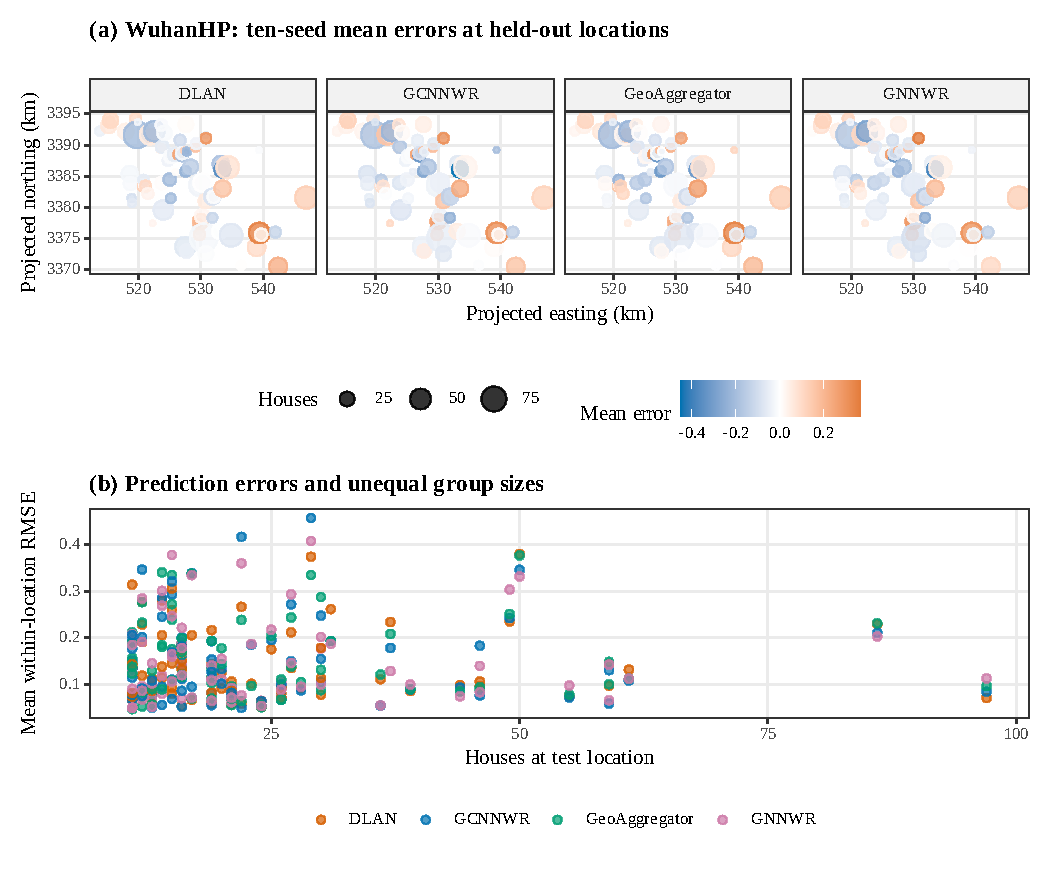
\includegraphics[width=\linewidth]{matched_hp_groups.pdf}
\caption{WuhanHP ten-seed mean residuals at held-out communities
and mean within-community RMSE against community size.
Marker size in the maps represents the number of houses.}\label{fig:hpgroups}
\end{figure}

The fitted planar DLAN retains coordinate-specific projections and adaptive retrieval,
with $D=2$ and $K=512$.
The two mean bandwidths, 0.0859 and 0.0861, are nearly equal,
which is compatible with an approximately isotropic Gaussian prior.
This is not an imposed restriction of the completed experiment;
content and learnt geographical biases remain active.

\subsection{GVI: nonlinear prediction and the added month coordinate}\label{sec:gvi3d}
For planar GVI, DLAN achieves RMSE $0.0985\pm0.0038$,
compared with $0.1066\pm0.0051$ for \GAgg,
$0.1185\pm0.0001$ for GCNNWR
and $0.1258\pm0.0255$ for GNNWR.
DLAN wins every paired seed against all three baselines.
Mean MAE is 0.0760 and mean $R^2$ is 0.3306,
compared with GNNWR's 0.0987 and $-0.1320$.
The fixed features, labels and spatial partitions are common to these models.

The OLS predictor recovered from GCNNWR's fitted coefficient buffers
has RMSE 0.1186 and $R^2=0.0297$.
GCNNWR's corresponding values of 0.1185 and 0.0318
show little improvement over this global linear reference.
DLAN and \GAgg have lower errors,
with the larger gain obtained by DLAN.
Figure~\ref{fig:gvi} compares prediction behaviour across the response range.
The results support flexible reference-conditioned prediction of visible greenery,
without isolating the nonlinear head from the remaining architecture.

\begin{figure}[tp]\centering
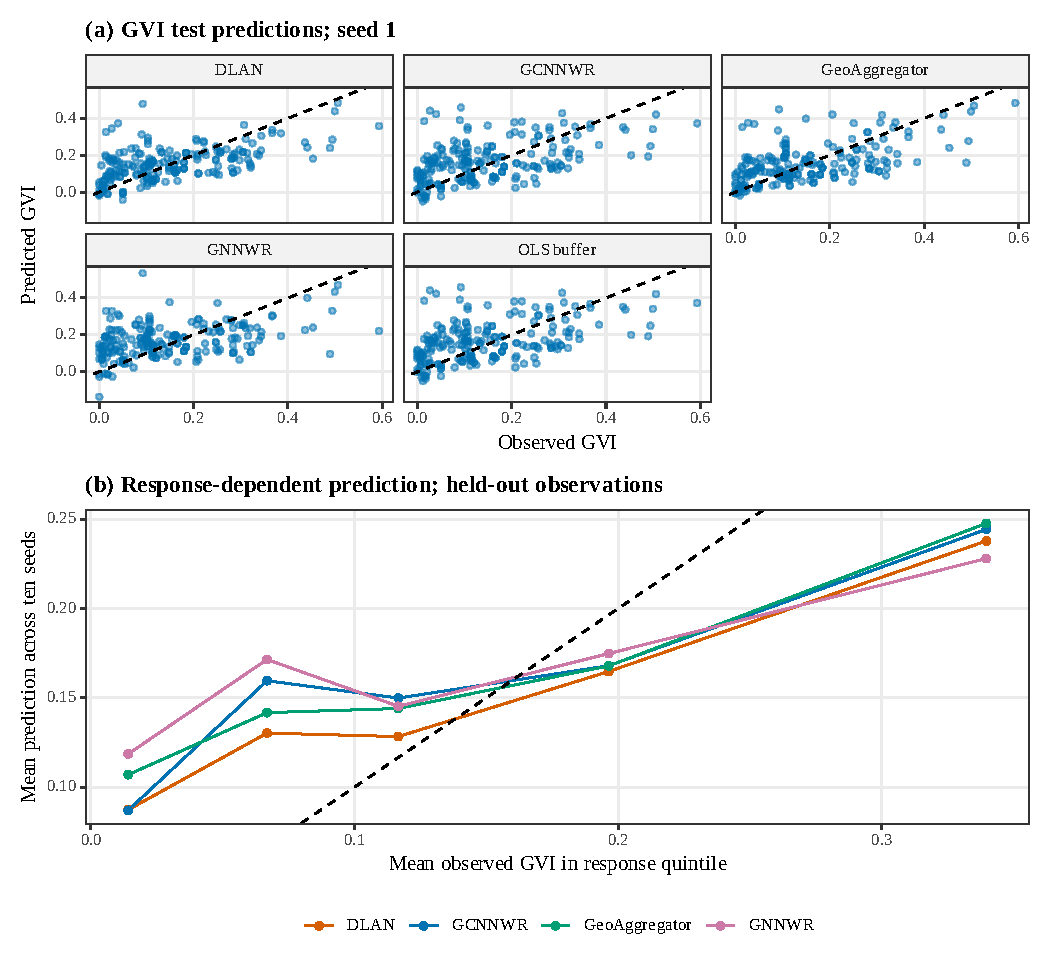
\includegraphics[width=\linewidth]{matched_gvi_response.pdf}
\caption{GVI seed-1 prediction diagnostics for all four planar models
and the recovered OLS predictor,
with ten-seed mean predictions summarised by observed-response quintile.
The quintiles are descriptive and do not enter training.}\label{fig:gvi}
\end{figure}

Adding elapsed capture month produces small mean improvements
(Table~\ref{tab:gvi3d}).
DLAN's RMSE falls from 0.09848 to 0.09613, a 2.39\% reduction;
\GAgg's falls from 0.10655 to 0.10498, a 1.47\% reduction.
The three-coordinate configuration wins six paired seeds for DLAN
and five for \GAgg (Figure~\ref{fig:gvi3d}).
The change is therefore not consistently beneficial across initialisations.
It is also accompanied by width adjustments,
and by a larger DLAN candidate budget.
The completed result is an equal-parameter three-coordinate configuration comparison,
not a pure intervention on temporal information.

\begin{table}[tb]\centering
\caption{GVI month augmentation under the same spatial split and 6,957-parameter budget.
The last column counts seeds with lower three-coordinate test RMSE.}\label{tab:gvi3d}
\small\begin{tabular}{lrrr}\toprule
Model & Planar RMSE & Month-augmented RMSE & Wins\\\midrule
DLAN & $0.09848\pm0.00376$ & $0.09613\pm0.00563$ & 6/10\\
\GAgg & $0.10655\pm0.00505$ & $0.10498\pm0.00621$ & 5/10\\\bottomrule\end{tabular}\end{table}

\begin{figure}[tp]\centering
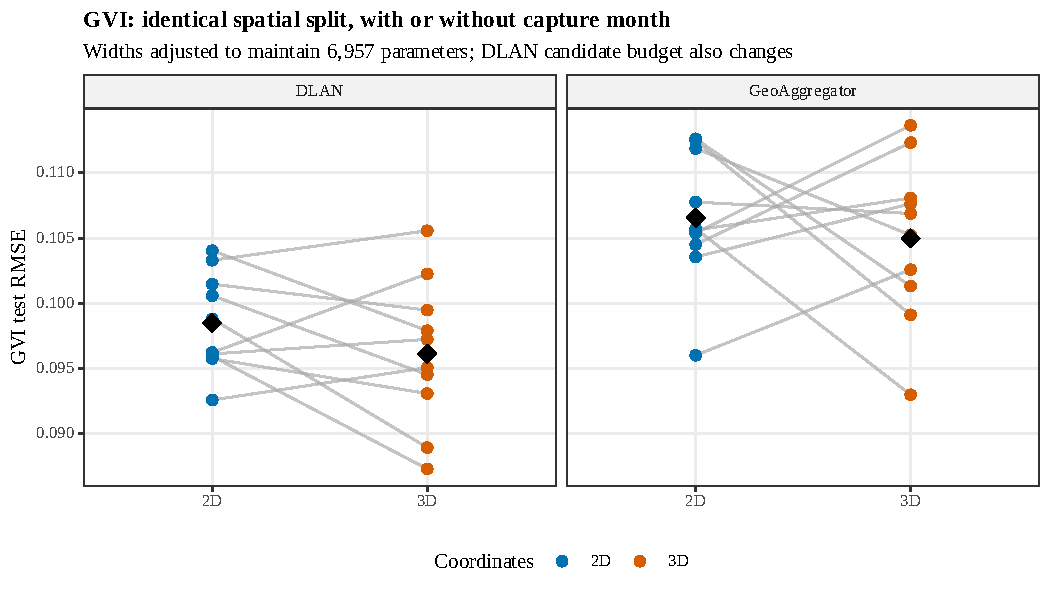
\includegraphics[width=\linewidth]{gvi_2d_3d.pdf}
\caption{Planar versus month-augmented GVI prediction on identical spatial partitions.
Lines connect paired seeds;
black diamonds indicate means.
All regressors have 6,957 parameters,
with architecture and candidate-count adjustments described in the text.}\label{fig:gvi3d}
\end{figure}

Both GVI experiments retain the original exploratory spatial split
and its overlapping image footprints.
The three-coordinate experiment does not predict a held-out future period.
Its smaller mean error supplies evidence for this particular augmented configuration,
rather than temporal extrapolation.

\subsection{Attention width and candidate support}\label{sec:odsensitivity}
Increasing WuhanOD attention width from 12 to 16,
with the $(10,8)$ prediction head retained,
raises the parameter count by 52.40\% to 10,773.
Mean RMSE changes only from 608.73 to 609.93,
whilst MAE rises from 52.08 to 52.94.
The seed standard deviation falls from 252.45 to 104.63,
and the worst-seed RMSE falls from 1,222.61 to 753.40.
However, the median rises from 552.52 to 635.55,
and width 16 wins only three paired seeds.
Additional width reduces the observed extreme failure,
but does not improve average or typical-run RMSE.

Mean $R^2$ rises from 0.8809 to 0.8937,
which is compatible with nearly unchanged mean RMSE:
the former averages squared-error-based scores,
whereas the latter averages their square roots.
The log-count RMSE improves from 0.4664 to 0.4563,
without a corresponding reduction on the count-scale criterion.
The default width-12 configuration therefore remains the smaller configuration
with better median RMSE and MAE.

\begin{table}[tb]\centering
\caption{Completed WuhanOD width and support experiments, ten seeds per configuration.
The K512 and K2048 configurations were run on another machine.}\label{tab:sensitivity}
\small\setlength{\tabcolsep}{4pt}\begin{tabular}{lrrrr}\toprule
Configuration & Parameters & RMSE & Median & Worst\\\midrule
Width 12; K1024 & 7,069 & $608.73\pm252.45$ & 552.52 & 1222.61\\
Width 16; K1024 & 10,773 & $609.93\pm104.63$ & 635.55 & 753.40\\
Width 12; K512 & 7,069 & $565.28\pm154.31$ & 556.20 & 827.76\\
Width 12; K2048 & 7,069 & $587.60\pm171.15$ & 563.58 & 840.72\\\bottomrule\end{tabular}\end{table}

The complete candidate-count runs have mean RMSE 565.28 at $K=512$,
608.73 at $K=1,024$ and 587.60 at $K=2,048$.
The smallest support has a mean 7.14\% below the reused baseline,
but wins only four paired seeds;
$K=2,048$ wins five.
Their medians, 556.20 and 563.58, remain above the baseline median of 552.52.
Thus more references do not yield monotonic improvement,
and a lower mean need not imply better performance in most runs
(Figure~\ref{fig:odsensitivity}).
Since $K=512$ and $K=2,048$ were run on another computer,
their relative times are not a candidate-count speed benchmark.
The experiments do not automatically change the default configuration
according to the reused test set.

\begin{figure}[tp]\centering
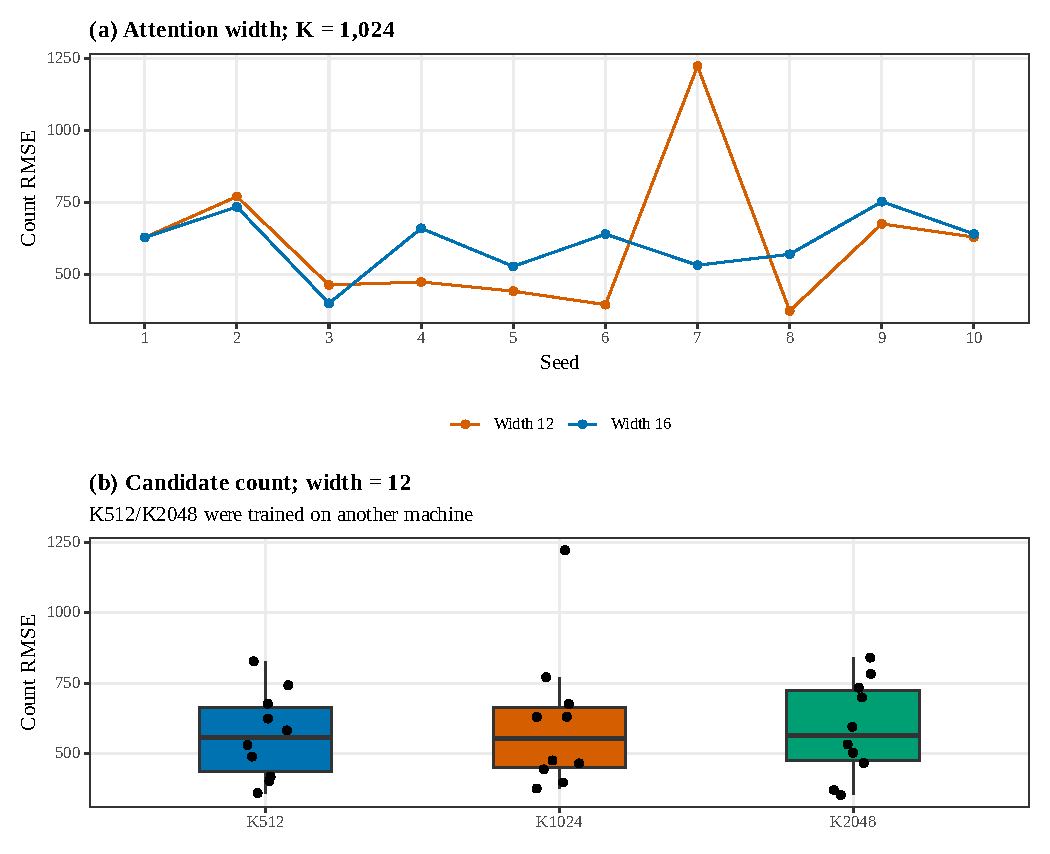
\includegraphics[width=\linewidth]{od_width_neighbours.pdf}
\caption{Completed WuhanOD width and candidate-support comparisons.
Top: paired width-12 and width-16 results at $K=1,024$.
Bottom: ten seeds per candidate count at width 12;
$K=512$ and $K=2,048$ were trained on another computer.}\label{fig:odsensitivity}
\end{figure}

The historical HPC product-distance model achieves
RMSE $497.16\pm117.28$ with width 12 and $K=1,024$.
Its core model and reference-trainer source files match the local implementation,
and its network shapes match the 7,069-parameter local model.
The execution protocols differ:
HPC uses a common coordinate scale and microbatches of 16,
whereas the local comparison uses per-axis standardisation and microbatches of 64.
Software and hardware also differ.
These historical scores therefore remain a separate protocol result,
not a replacement for the local parameter-matched ranking.
The coordinate-scale and microbatch cross-diagnostic is incomplete
in the frozen evidence snapshot and supplies no final attribution here.

\subsection{Computational cost and dimensional extensibility}
The expanded fit-cost table includes the completed GNNWR/GTNNWR baselines
(Table~\ref{tab:cost}).
DLAN and \GAgg have similar mean \COO fit times,
79.56 and 80.80 seconds;
GTNNWR is faster at 41.32 seconds, with higher error.
For WuhanHP, GNNWR and DLAN have comparable mean costs,
32.41 and 33.90 seconds,
whilst GCNNWR is faster at 13.17 seconds.
On GVI, DLAN takes 5.16 seconds,
below \GAgg's 6.41 and GNNWR's 9.25,
but above GCNNWR's 0.65.
The accuracy--cost trade-off depends on the task
(Figure~\ref{fig:cost}).

\begin{table}[tb]\centering
\caption{Recorded mean fit cost for the reported configurations.
WuhanOD DLAN K512 was trained on another machine;
its 804.63-second time is not a same-hardware comparison with the baselines.}\label{tab:cost}
\small\begin{tabular}{llrr}\toprule
Case & Model & Fit seconds & Epochs\\\midrule
\COO & DLAN & 79.56 & 126.4\\
 & \GAgg & 80.80 & 170.1\\
 & GTNNWR & 41.32 & 210.6\\
\midrule
WuhanOD & DLAN & 804.63 & 230.4\\
 & \GAgg & 305.22 & 268.7\\
 & GNNWR & 33.83 & 262.2\\
\midrule
WuhanHP & DLAN & 33.90 & 40.3\\
 & \GAgg & 45.45 & 62.2\\
 & GNNWR & 32.41 & 120.5\\
 & GCNNWR & 13.17 & 88.0\\
\midrule
GVI & DLAN & 5.16 & 56.6\\
 & \GAgg & 6.41 & 75.2\\
 & GNNWR & 9.25 & 219.0\\
 & GCNNWR & 0.65 & 32.1\\\bottomrule\end{tabular}\end{table}

\begin{figure}[tp]\centering
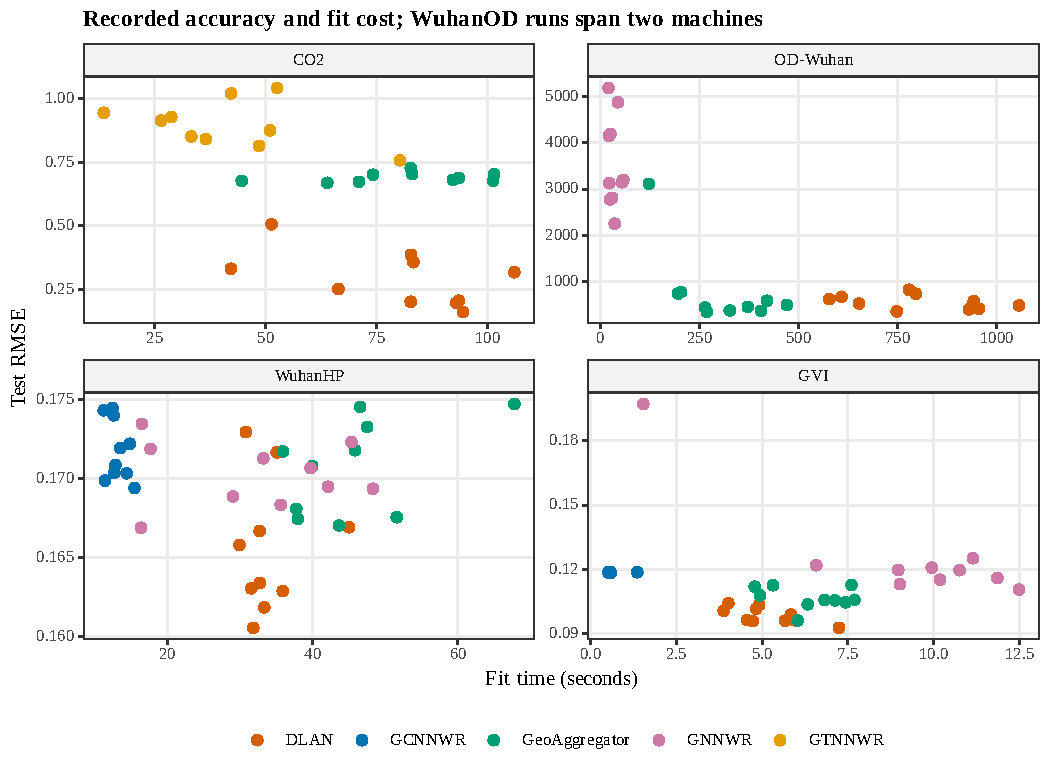
\includegraphics[width=\linewidth]{matched_accuracy_cost.pdf}
\caption{Recorded fit cost and test RMSE for the 140 reported fits.
WuhanOD K512 uses the second machine, so its time is not directly comparable.
Final prediction export and checkpoint-reload auditing are outside the fit timer.
Case-specific axes retain the different response scales.}\label{fig:cost}
\end{figure}

Fit cost includes the stopping trajectory,
so it is distinct from computation per epoch.
In the retained K1024 diagnostic at 7,069 parameters,
DLAN, \GAgg and GNNWR take means of 269.36, 305.22 and 33.83 seconds,
respectively.
The rapid coefficient-modulation baseline is also the least accurate in that group.
Some flow runs reach the 300-epoch cap;
these timings do not establish that every configuration has converged to its attainable optimum.

The architecture accommodates two, three and four coordinates
without constructing a regular grid over every coordinate combination.
Coordinate-indexed projections grow with $D$,
whereas a $q$-bin grid on each axis would contain $q^D$ cells.
This dimensional extensibility does not remove exact reference search.
The current retrieval scans all training references and performs stable sorting,
with $N_{\train}D$ coordinate-distance work per query, block and head
(Figure~\ref{fig:complexity}).
Restricted attention controls subsequent attention activation size;
it does not establish subquadratic end-to-end training in sample size.

\begin{figure}[tp]\centering
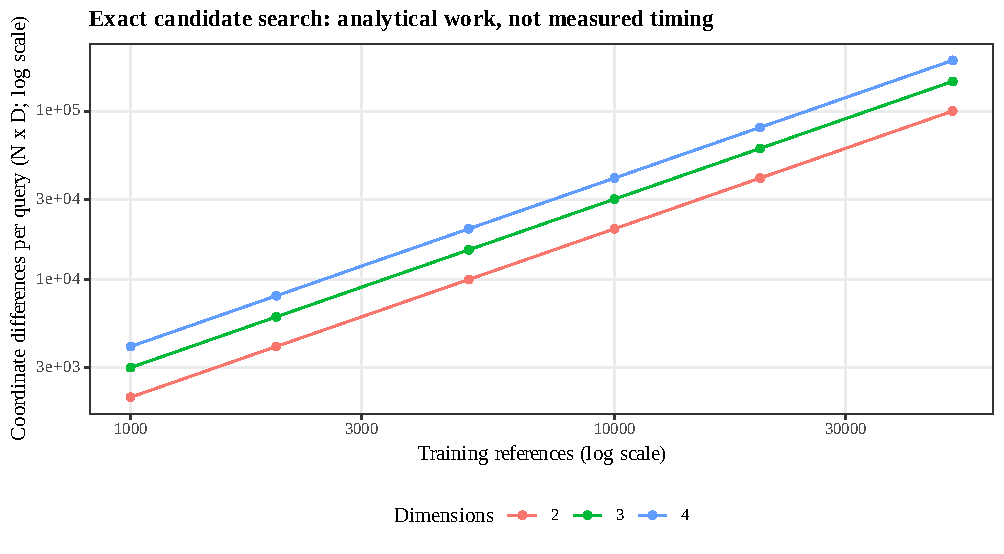
\includegraphics[width=.94\linewidth]{retrieval_complexity.pdf}
\caption{Analytical distance work per query, $N_{\train}D$,
for one block and head.
Stable sorting and neural projections add computation;
these curves are not empirical timing measurements.}\label{fig:complexity}
\end{figure}

\section{Discussion}\label{sec:discussion}
\subsection{Predictive scope under controlled capacity}
The completed baselines strengthen the evidence for DLAN
on subsequent-year \COO, community-held-out housing and planar GVI prediction.
Its advantage on these cases persists against GNNWR/GTNNWR,
whose learned proximity functions retain coefficient-wise OLS modulation.
The distinction is in the response construction:
DLAN combines a nonlinear query-covariate path with reference-derived conditioning,
whereas these baselines retain a position-specific linear combination of covariates.
The measured scores compare complete information-processing systems,
including their different uses of training responses.
They do not isolate nonlinearity or reference labels as the sole source of the gain.

The WuhanOD results show why a single total parameter count is insufficient
to characterise a neural spatial predictor.
The superseded narrow-allocation model is inferior to \GAgg;
restoring attention width and reporting the completed K512 configuration
yields the lower mean RMSE of 565.28.
Its median and paired seed wins still do not favour DLAN.
Increasing attention width further does not improve mean RMSE,
and increasing candidate support does not yield monotonic improvement.
There is therefore no supported rule that more attention capacity
or more reference observations will always improve flow prediction.
The distribution across seeds, the target scale and the allocation of parameters
all affect the practical comparison.

\subsection{Coordinate scales and geometric meaning}
The \COO checkpoints learn a wider temporal scale than spatial scales,
providing a fitted description of the geographical prior used for this panel.
These are coordinate-, head- and block-specific parameters,
rather than MGWR covariate-specific coefficient bandwidths.
They govern locality and candidate access;
they do not directly identify the spatial or temporal scale of an individual covariate effect.

Coordinate preprocessing is also a model choice.
For WuhanOD's four projected spatial coordinates,
a common scale preserves the relative metric of equal physical displacements across axes.
Per-axis standardisation instead measures displacement relative to each axis's sample dispersion.
For space--time data with different units,
separate coordinate transformations make those units numerically comparable.
Neither construction is a universal metric for every geographical object.

If only the Gaussian kernel were retained,
a change in coordinate scale could be compensated by a corresponding bandwidth change.
The full network also uses Fourier coordinate encoding and learnt offset biases,
so rescaling coordinates alters additional inputs.
Likewise, an equal effective optimisation batch does not make two microbatch sizes identical:
dropout draws and floating-point accumulation can follow different paths.
The matching network architecture in the HPC and local runs
therefore does not imply identical training conditions or predictions.
The unfinished cross-diagnostic is needed to separate these effects.

\subsection{Planar and spatio-temporal environmental prediction}
WuhanHP demonstrates prediction in grouped data without requiring a group identifier
or a fitted random-effect distribution.
Training-reference context supplies a geographical condition,
whilst individual dwelling covariates preserve within-community variation.
The equal-community result shows that the leading mean accuracy
is not confined to the weight given to large communities.
Its nearly equal planar bandwidths are compatible with a simple isotropic prior,
but the completed experiment does not impose the DLAN-P restriction.

The planar GVI result supports nonlinear local prediction from a common environmental representation.
GCNNWR changes the global OLS diagnostic little,
whereas both attention-based predictors lower error,
with DLAN providing the strongest result in the main comparison.
The completed month-augmented experiment supplies a modest further mean reduction,
but not a consistent advantage across seeds.
Widths and DLAN candidate count change to preserve the parameter budget,
so the comparison does not isolate temporal information alone.
The inherited exploratory split and overlapping image footprints apply to both versions.
A buffered spatial evaluation or future-month holdout would test different prediction supports.

\subsection{FiLM conditioning and evidence for individual modules}\label{sec:ablations}
DLAN and \GAgg both use training-reference information,
but introduce the resulting context into prediction differently.
\GAgg concatenates the aggregated representation with query attributes
before its nonlinear readout.
DLAN uses the local condition to generate layer-wise scaling and translation,
modulating the intermediate query-attribute representation through FiLM.
This explicitly parameterises a multiplicative interaction between context and hidden features.
A concatenation network can also learn interactions;
FiLM supplies a distinct conditioning structure rather than a guarantee of higher accuracy.

The completed width and candidate experiments assess configuration sensitivity,
not the isolated contribution of FiLM.
A direct comparison would retain the candidate identifiers and attention condition,
then replace only the modulated head with an appropriate capacity-controlled alternative.
Similarly, removing response encoding would test the value of labelled reference context.
Flexible tree ensembles would supply additional controls for nonlinear tabular prediction
\citep{Breiman-2001,Friedman-2001,ChenGuestrin-2016,FriedmanPopescu-2008}.
These interventions have not been completed for final DLAN.

The historical joint-attention Gaussian experiment remains separate.
Removing its Gaussian term increases mean test RMSE
from 0.161806 to 0.164707 on WuhanHP,
and from 804.52 to 832.66 on WuhanOD,
across three paired seeds.
The increases are 1.79\% and 3.50\%
(Figure~\ref{fig:ablation}).
This supports retaining the prior in that tested configuration,
without making it an isolated ablation of current DLAN retrieval.

\begin{figure}[tp]\centering
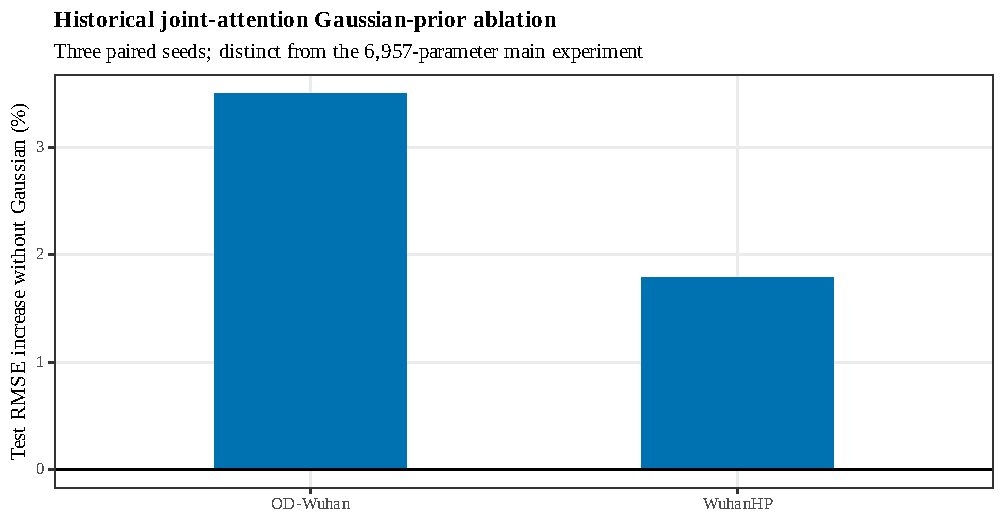
\includegraphics[width=.94\linewidth]{historical_gaussian_ablation.pdf}
\caption{Historical joint-attention Gaussian-prior ablation,
with three seeds and its original neighbourhood configuration.
The results are separate from the main and supplementary DLAN experiments.}\label{fig:ablation}
\end{figure}

Table~\ref{tab:ablation} distinguishes completed configuration comparisons
from interventions still needed for module attribution.
Attention weights describe the predictor's reference aggregation;
they do not automatically explain substantive causes of the response
\citep{JainWallace-2019,WiegreffePinter-2019}.

\begin{table}[tb]\centering
\caption{Status of component-related comparisons.
Completed configuration experiments do not replace the remaining module-isolating interventions.}\label{tab:ablation}
\small\begin{tabularx}{\linewidth}{lXX}\toprule
Component & Comparison & Evidence status\\\midrule
Capacity allocation & Width/head reallocation; width 12 vs 16 & Completed, ten seeds; budgets differ\\
Candidate support & $K=512,1,024,2,048$ & Completed, ten seeds; cross-machine baseline retained\\
Temporal coordinate & GVI planar vs month-augmented & Completed, ten seeds; widths and support adjusted\\
Coordinate preprocessing & Common vs per-axis scale and microbatch & Cross-diagnostic incomplete\\
Reference retrieval & Euclidean vs bandwidth-scaled at fixed $K$ & Module-isolating comparison not completed\\
Attention terms & Tied scales; omitted content or directional bias & Module-isolating comparisons not completed\\
Reference response & Include vs omit response encoding & Not completed\\
Prediction head & FiLM vs matched concatenation/linear head & Not completed\\\bottomrule
\end{tabularx}\end{table}

\subsection{Generality and computational development}
The same locality construction handles planar, space--time and endpoint objects,
with task-dependent predictive outcomes.
The reported configurations give DLAN the lowest mean RMSE on all four cases,
whilst the flow experiments expose sensitivity to capacity allocation,
seed variation, candidate support and execution protocol.
The completed month-augmented GVI result adds a small positive mean comparison,
not evidence of future-time extrapolation.
These findings define the model's present predictive scope more clearly
than a claim of uniform superiority.

Exact reference search remains a computational bottleneck.
Partial selection, batched distance kernels or dynamic metric indexing
could reduce its cost,
but require a common-hardware benchmark including retrieval,
training, prediction and peak memory.
Rolling \COO evaluation, endpoint-held-out flows and buffered GVI partitions
would extend the assessment to new inference supports
\citep{RobertsBahn-2017,ValaviElith-2019}.
These follow from the current protocol differences,
rather than being unreported results of the existing fits.

\section{Conclusion}\label{sec:conclusion}
DLAN combines coordinate-specific geographical scales,
bandwidth-adaptive reference access and nonlinear conditional prediction.
Its attention integrates content similarity, learnt geographical bias
and a Gaussian product prior over shared candidate identifiers.
The resulting condition modulates query attributes through FiLM.
The construction accommodates planar, space--time and geographical-flow coordinates.

The reported comparison contains fourteen configurations with ten seeds each.
Regressors use 6,957 parameters for \COO, WuhanHP and GVI,
and 7,069 for the restored-width WuhanOD comparison.
The selected WuhanOD DLAN uses 512 reference candidates,
with mean RMSE $565.28\pm154.31$.
The corresponding K2048 experiment yields $587.60\pm171.15$;
the earlier 919.92 score describes a superseded narrow-allocation configuration.
Relative to the stated \GAgg baselines,
DLAN reduces mean RMSE by 57.81\%, 26.85\%, 2.99\% and 7.58\%
on \COO, WuhanOD, WuhanHP and planar GVI, respectively.
The WuhanOD mean advantage coexists with a higher median,
four wins in ten paired seeds and a cross-machine execution difference.
Thus the result supports the reported mean prediction performance,
whilst retaining the distinction between configuration choice,
seed-sensitive risk and controlled computational comparison.

\section*{Data and code availability}
The research repository contains model implementations, fixed data contracts,
saved predictions, checkpoint-reload audits and configuration hashes.
The article directory contains the R plotting script,
metric-recalculation script and the evidence tables used in the manuscript.
The reported comparison combines the retained matched-case results
with the pinned upstream baselines and the selected width-12 K512 WuhanOD model.
The source of every reported configuration is recorded in
\texttt{reported\_configuration\_manifest.json}.
Supplementary outputs retain their own configuration and execution metadata.
The GVI features are inherited from a frozen preparation pipeline;
source datasets are not redistributed by the article build.
A public repository address, dataset permissions and persistent identifiers
will be supplied before submission.
\section*{Disclosure statement}
\pending{Authors to provide the conflict-of-interest declaration.}
\section*{Funding}
\pending{Authors to provide funding information.}
\section*{Author contributions}
\pending{Authors to confirm names, affiliations and contributions.}
\printnoidxglossary[type=\acronymtype,title={Abbreviations}]
% Bibliography entries are read from the user-supplied Zotero export.
\bibliographystyle{tfcad}
\bibliography{zotero}
\end{document}
